\documentclass{article}
\usepackage[utf8]{inputenc}

% Basic packages
	\usepackage{amssymb}
	\usepackage{amsmath}
	\usepackage{graphicx}
	\usepackage[czech]{babel}
	\usepackage{natbib}

% Relevant packages
	\usepackage{bm}
	\usepackage{bbm}
	\usepackage{geometry}
	\usepackage{enumitem}
	\usepackage{listings}
	\usepackage{multicol,float}
	\usepackage{hyperref}

% Document settings
	\geometry{a4paper,margin=15mm}

	\setlist[itemize]{nolistsep,noitemsep}
		
	\setlength{\parindent}{0pt}
	\setlength{\parskip}{1.5em}
	\renewcommand{\baselinestretch}{1.2}

	\setlength{\abovedisplayskip}{1.2em}
	\setlength{\belowdisplayskip}{1.2em}
	\renewcommand{\arraystretch}{1.2}

\begin{document}
	\section{Základní pojmy optimalizace. Vysvětlit a popsat pojmy: cílová funkce, gradient, Hessova matice, optimalizační proměnné, lokální extrém a lokální optimalizace, globální extrém a globální optimalizace, jednokriteriální a vícekriteriální optimalizace, Pareto množina.}

	\section{Simplexová (polytopová) optimalizační metoda – popis algoritmu.}

	\section{Rosenbrockova optimalizační metoda – popis algoritmu.}
	
	\section{Základní principy globální optimalizace pomocí genetických algoritmů.}

	\section{Základní principy globální optimalizace pomocí simulovaného žíhání.}

	\section{Kinematická syntéza převodových mechanismů (ilustrace na tříbodové a čtyřbodové syntéze klikového mechanismu).}

	\subsection*{3 body přesnosti}
	\begin{equation}
	l^{2}=\left(\xi_{B}-\xi_{A}\right)^{2}+\left(\eta_{B}-\eta_{A}\right)^{2}= s^{2}+r^{2} \cos ^{2} \varphi-2 r \cos \varphi+e^{2} + r^{2} \sin ^{2} \varphi-2 r \sin \varphi
	\end{equation}
	upravíme na
	\begin{equation}
		2 r s \cos \varphi+2 r \sin \varphi-\left(r^{2}-l^{2}+e^{2}\right)=s^{2}
	\end{equation}
	pomocné proměnné
	\begin{align}
		b_{1} &= 2 r \\
		b_{2} &= 2 r e \\
		b_{3} &= r^{2}-1^{2}+e^{2}
	\end{align}

	\begin{figure}[h!]
		\centering
		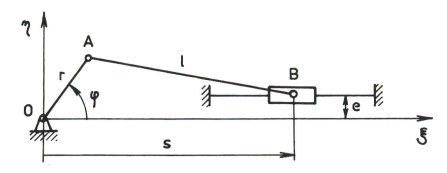
\includegraphics{figs/KlikovyMechanismus.png}
	\end{figure}

	\url{https://moodle-vyuka.cvut.cz/pluginfile.php/242037/mod_resource/content/0/se_tremi.pdf}

	\subsection*{4 body přesnosti}
	\begin{figure}[h!]
		\centering
		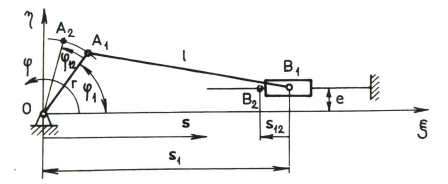
\includegraphics{figs/KlikovyMechanismus4.png}
	\end{figure}

	\url{https://moodle-vyuka.cvut.cz/pluginfile.php/242038/mod_resource/content/0/se_ctyrmi.pdf}

	\section{Formulace cílové funkce a optimalizační úlohy syntézy vodícího čtyřkloubového mechanismu.}

	\section{Kinematická syntéza vybraného prostorového mechanismu.}

	\section{Obecné úlohy kinematické syntézy mechanismů s více stupni volnosti, optimalizace manipulovatelnosti a zástavbového prostoru (ilustrace na zvoleném příkladu).}

	Manipulovatelnost je definována jako
	\begin{equation}
		\bm{D} = \frac{1}{\operatorname{cond}(\bm{J})}
	\end{equation}
	kde $\operatorname{cond}(\bm{J})$ je podmíněnost Jakobiho matice určující převod mezi rychlostí pohonů $\bm{v}_p$ a end-effektoru mechanismu $\bm{v}_e$.
	\begin{equation}
		\bm{v}_p = \bm{J} \bm{v}_e
	\end{equation}
	a také určuje převod akčních sil $\bm{F}_p$ a sil působících na koncový bod $\bm{F}_e$
	\begin{equation}
		\bm{F}_e = \bm{J} \bm{F}_p
	\end{equation}

	Podmíněnost lze definovat přes svd rozklad
	\begin{equation}
		\operatorname{cond}(\bm{J}) = \frac{s_{max}}{s_{min}}
		\;,\quad 
		\bm{J} = \bm{U} \bm{S} \bm{V}^T
		\;,\quad 
		\bm{S} = \operatorname{diagm}(s_i)
	\end{equation}

	\section{Metody řešení úloh kinematické syntézy – analytické řešení, použití optimalizačních metod, alternativní formulace. Vysvětlit problém řešitelnosti ve vztahu k různým typům formulací.}

	\begin{itemize}
	\item Analitické řešení
	\begin{itemize}
		\item závisý na odvození kinematických rovnic specifického mechanismu a jejich převod do tvaru, kde optimalizované parametry vystupují jako lineární koeficienty nebo je lze jinak (ad-hoc) vyjádřit
	\end{itemize}
	\item Použití optimalizačních metod
		\begin{itemize}
		\item postaveny kolem optimalizace kriteriální funkce
		\item fungují s kinematickými/vazbovými rovnicemi v libovolném tvaru
		\item numerické metody nám dávají velkou volnost co se týče formulace kritérií
		\end{itemize}
	\item Alternativní formulace
		\begin{itemize}
		\item např. metoda přidruženého disipativního modelu
		\end{itemize}
	\end{itemize}

	\subsection*{Řešitelnost vodících mech.}
	máme-li $p$ parametrů a $k$ bodů přesnosti s $n$ souřadnicemi. Mužeme obecně říct o problému jejich průchodu
	\begin{itemize}
		\item [$p<kn$] - můžeme se pouze přiblížit k řešení
		\item [$p=kn$] - máme jednoznačné řešení
		\item [$p>kn$] - máme nekonečně mnoho možných řešení (je vhodné například zavést další kritérium jako minimální rozměry mechanismu)
	\end{itemize}

	\subsection*{převodové mechanismy}
	Většinou zavislost rychlosti nebo polohy výstupu na vstupu v podobě spojité funkce (pro rychlost bývá konstanta) při splnění prostorových požadavků.

	\subsection*{ndof mechanismy}
	Maximalizace manipulovatelnosti při minimalizaci zástavbového prostoru

	\section{Kinematická syntéza pomocí přidruženého disipativního mechanismu.}
	\begin{enumerate}
		\item Uměle přidám mechanismu stupně volnosti, které mu umožní se dostat i do jinak nedosažitelných poloh.
		\item Stupňům přidám virtuální pružiny a tlumiče, tak minimalizovali jejich polohu
		\item Optimalizuju parametry mechanismu, tak aby bylo disipováno při simulaci minimální množství energie v přidaných stupních volnosti
	\end{enumerate}

	Optimální řešení by tedy mělo vykonat trajektorii bez posuvu v nově přidaných stupních volnosti a tedy je vůbec nevyžadovat.

	\section{Formulace a řešení globální dynamické úlohy mechanismů. }

	\section{Kalibrace mechanismů, základní algoritmus, kalibrovatelnost, volba kalibračních poloh. Formulace pro případ, kdy v rovnicích vystupují neměřené souřadnice.}

	\begin{equation}
		\bm{f}(\bm{x},\bm{p}) = \bm{0}
	\end{equation}
	kde $\bm{x}$ jsou měřené veličiny a $\bm{p}$ kalibrační parametry

	\begin{equation}
		\bm{F}(\bm{X},\bm{p})
		=
		\bm{0} \doteq \bm{F}(\bm{X},\bm{\overline{p}})
		+
		\underbrace{\frac{\partial \bm{F}(\bm{X},\bm{\overline{p}})}{\partial p}}_{\bm{J}_p} \Delta\bm{p}
		\;\Rightarrow\;
		\Delta\bm{p} = \bm{J}_p^+ \bm{F}(\bm{X},\bm{\overline{p}})
	\end{equation}
	kde
	\begin{equation}
		\bm{F}
		=
		\begin{bmatrix}
			\bm{f}(\bm{x}_1,\bm{p}) = \bm{0} \\
			\vdots \\
			\bm{f}(\bm{x}_n,\bm{p}) = \bm{0}
		\end{bmatrix}
		\;,\quad 
		\bm{X}
		=
		\begin{bmatrix}
			\bm{x}_1 \\
			\vdots \\
			\bm{x}_n
		\end{bmatrix}
	\end{equation}

	\subsection*{Kalibrovatelnost}

	Kalibrovatelnost je obcená schopnost kalibrovat mechanismus. Závisí na volbě kalibrovaných parametrů i kalibračních poloh.

	Při výše popsané metodě míru kalibrovatelnosti značně ovlivňuje podmíněnost matice $\bm{J}_p^T \bm{J}_p$.

	\section{Kalibrace mechanismu se zohledněním modelu chyb senzorů.}
	\begin{equation}
		\bm{f}(\bm{\overline{x}}+\bm{\hat{x}},\bm{\overline{p}}+\bm{\hat{p}}) = \bm{0}
	\end{equation}
	kde $\bm{\overline{x}}$ jsou měřené veličiny, $\bm{\hat{x}}$ opravy veličiny, $\bm{p}$ kalibrační parametry a $\bm{\hat{p}}$ opravy parametrů.

	Cílem následné optimalizace je minimalizovat kvadratické kritérium
	\begin{equation}
	\chi^2 = \sum_{i=1}^N \bm{\hat{x}}_i^T \bm{C}_x^{-1} \bm{\hat{x}}_i + \bm{\hat{p}}^T \bm{C}_p^{-1} \bm{\hat{p}} 
	\end{equation}
	pro $N$ měření, kde $\bm{C}_p$ je kovariace ``chyby'' parametrů a $\bm{C}_x$ signálů čidel, při splnění podmínky
	\begin{equation}
		\sum_{i=1}^N \bm{f}(\bm{\overline{x}}_i+\bm{\hat{x}}_i,\bm{\overline{p}}+\bm{\hat{p}}) = \bm{0}
	\end{equation}

	Základní metodou řešení těchto problemů je \emph{Lagrangeova metoda} postavená na zavedení Lagrangiánu, v našem případě
	\begin{equation}
		L = \chi^2 + \sum_{i=1}^N \bm{\lambda}_i \bm{f}(\bm{\overline{x}}_i+\bm{\hat{x}}_i,\bm{\overline{p}}+\bm{\hat{p}})
	\end{equation}
	\emph{First-Order Conditons} neboli podmínky prvního řádu, které zaručují nalezení lokálního extrému při splnění podmínky lze zapsat jako
	\begin{align}
		\frac{\partial L}{\partial \bm{\hat{x}}_i} &= \bm{0} \\
		\frac{\partial L}{\partial \bm{\hat{p}}} &= \bm{0} \\
		\frac{\partial L}{\partial \bm{\lambda}_i} &= \bm{0}
	\end{align}

	\url{https://www.econgraphs.org/textbook/math/optimization/constrained}
	
	Krivošej ve své bakalářce odvozuje převod, který umožnuje řešit tuto soustavu rovnic bez potřeby výpočtu druhé derivace, ale vzhledem k rozšířenosti různých metod pro numerickou diferenciaci a obecných řešičů omezených optimalizačních problémů mi přijde zbytečné ji popisovat.

	\url{https://dspace.cvut.cz/bitstream/handle/10467/65598/F2-BP-2016-Krivosej-Jan-Kinematicka%20kalibrace%20zohlednujici%20rozlozeni%20chyb%20cidel.pdf?sequence=1&isAllowed=y}

	\section{Kalibrace mechanismů, implementace na prostorový seriový robotický řetězec. Zavedení kalibračních parametrů a maticové formulace s nimi.}

	Přechod mezi následujícími osami lze popsat 4 parametry
	\begin{itemize}
		\item Denavit-Hartenbergovy parametry $h$,$\beta$,$d$,$\phi$
		\item Beneš-Šikovy parametry $x_1$,$x_2$,$\phi_1$,$\phi_2$
	\end{itemize}

	\begin{align}
		&\underbrace{
			\bm{T}_x(x_0)\bm{T}_y(y_0)\bm{T}_z(z_0)\bm{T}_{\phi_x}(\phi_{x_0})\bm{T}_{\phi_y}(\phi_{y_0})\bm{T}_{\phi_z}(\phi_{z_0})
		}_{\text{Tracker-Základna}}
		\bm{T}_{\phi_z}(\phi_{12})
		\underbrace{
			\bm{T}_x(x_2)\bm{T}_z(z_2)\bm{T}_{\phi_x}(\phi_{x_2})\bm{T}_{\phi_z}(\phi_{z_2})
		}_{\text{Kalibrace na tělesu 2}}\\&
		\bm{T}_{\phi_x}(-\phi_{23})
		\underbrace{
			\bm{T}_x(x_3)\bm{T}_z(z_3)\bm{T}_{\phi_x}(\phi_{x_3})\bm{T}_{\phi_z}(\phi_{z_3})
		}_{\text{Kalibrace na tělesu 3}}
		\ldots
		\bm{r}_{N K} = \bm{r}_{0K}
	\end{align}
	(pls někdo doplňte zbytek rovnice a obrázek)

	Pro každou kalibrační polohu máme 3 rovnice a mechanismus má dohromady 27 kalibračních parametrů $\Rightarrow$ potřebujeme min. 9 kalibračních poloh.

	Ještě je otázkou jestli na transformaci mezi trackerem a základnou použít 4 (osa - osa), 5 (těleso - bod+osa) nebo 6 (těleso - těleso) parametrů. Také mi přijde, že zde nejsou kalibrovány počáteční odchylky natočení $\phi_{12_0}$, $\phi_{23_0}$.

	\section{Identifikace pomocí modelů unifikované struktury a pomocí ad-hoc modelů. Vysvětlit na příkladu použití optimalizace pro identifikaci.}

	\section{Použití optimalizačních metod pro syntézu zákona řízení. Ilustrace na příkladu řízeného tlumiče. Výhoda poloaktivních konceptů při optimalizaci.}

\end{document}